\section{Frontend}
\begin{frame}
    \frametitle{Frontend}
    \begin{columns}
        \begin{column}{0.48\textwidth}
            \begin{itemize}
                \item TypeScript als Programmiersprache
                \item Vue.js für UI-Komponenten
                \item Vuex für Zustandsverwaltung und unidirektionalen Datenfluss
                \item Bibliothek für STOMP oder MQTT (Verbindung zu RabbitMQ)
            \end{itemize}
        \end{column}
        \begin{column}{0.48\textwidth}
            \begin{figure}
                \centering
                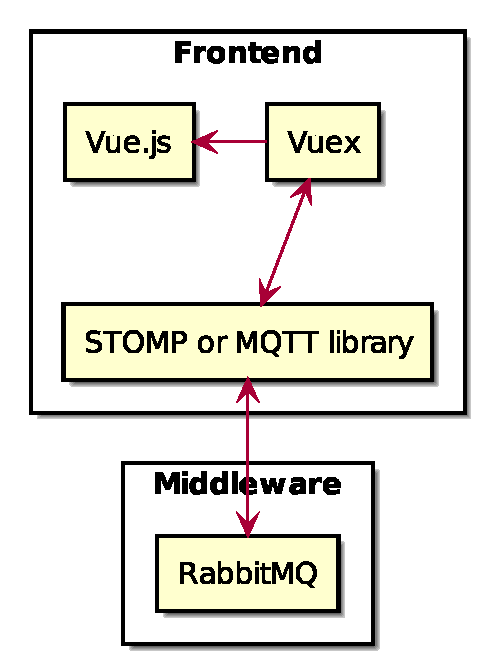
\includegraphics[height=6cm]{media/Frontend.eps}
            \end{figure}
        \end{column}
    \end{columns}
\end{frame}

\begin{frame}
    \frametitle{Vue.js}
    \begin{columns}
        \begin{column}{0.68\textwidth}
            \begin{itemize}
                \item Frontend Framework für UI-Komponenten
                \item Vergleichbar mit React (Virtual DOM, usw.)
                \item Komponenten erweitern HTML-Elemente über Direktiven
            \end{itemize}
        \end{column}
        \begin{column}{0.28\textwidth}
            \begin{figure}
                \centering
                
\includegraphics[height=3cm]{media/Vue-JS-01.eps}
            \end{figure}
        \end{column}
    \end{columns}
\end{frame}

\begin{frame}
    \frametitle{Vuex}
    \begin{columns}
        \begin{column}{0.58\textwidth}
            \begin{itemize}
                \item Ein einziger Datenspeicher als \textit{Single Source of Truth}
                \item Vergleichbar mit Redux
                \item Daten fliessen immer in eine Richtung
                \item Aktionen (User-Interaktion, Messages, usw.) verändern den Zustand, was zu einer Aktualisierung des GUI führt.
            \end{itemize}
        \end{column}
        \begin{column}{0.38\textwidth}
            \begin{figure}
                \centering
                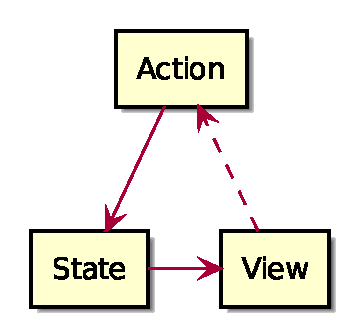
\includegraphics[height=4cm]{media/Vuex.eps}
            \end{figure}
        \end{column}
    \end{columns}
\end{frame}